\section{抛物线与屋顶}
\markboth{7. 抛物线与屋顶}{7. 抛物线与屋顶}

\noindent
\begin{minipage}[t]{0.43\textwidth}
  \centering
  \vspace{-2pt}
  \begin{tikzpicture}[scale=0.76]
    \def\px#1#2{1.0*(#1) + 0.85*(#2)}
    \def\py#1#2{0.22*(#1) - 0.48*(#2) - 0.35*(#1)*(#1) - 0.25*(#2)*(#2)}

    \draw[line width=0.65pt]
      plot[domain=-1:1, samples=25] ({\px{-1}{\x}}, {\py{-1}{\x}});
    \draw[line width=0.65pt]
      plot[domain=-1:1, samples=25] ({\px{1}{\x}}, {\py{1}{\x}});
    \foreach \vv in {-1, 0, 1} {
      \draw[line width=0.7pt, curveblue, domain=-1:1, samples=30]
        plot ({\px{\x}{\vv}}, {\py{\x}{\vv}});
      \draw[line width=0.5pt] ({\px{-1}{\vv}}, {\py{-1}{\vv}}) -- ({\px{1}{\vv}}, {\py{1}{\vv}});
    }
    \node[below, font=\scriptsize] at ({\px{-0.30}{-1}}, {\py{-0.30}{-1}-0.02}) {$a$};
    \node[below, font=\scriptsize] at ({\px{-0.32}{0}}, {\py{-0.32}{0}-0.03}) {$a$};
    \node[below, font=\scriptsize] at ({\px{0.35}{1}}, {\py{0.35}{1}-0.05}) {$a$};
    \draw[line width=0.85pt, black, domain=-1:1, samples=30]
      plot ({\px{0}{\x}}, {\py{0}{\x}});
    \node[above right=-2pt, font=\scriptsize] at ({\px{0}{-0.20}}, {\py{0}{-0.20}}) {$b$};

    \draw[-{Stealth[length=5pt]}, line width=1.4pt]
      (-0.9, 0.65) .. controls (-0.1, 0.95) and (0.55, 0.65) .. (1.05, 0.12);
    \node[above, font=\scriptsize] at (0.12, 0.86) {曲线 $a$ 沿曲线 $b$ 平行移动};
  \end{tikzpicture}
  \par\vspace{4pt}{\footnotesize 图\ 7.1}
\end{minipage}
\hfill
\begin{minipage}[t]{0.53\textwidth}
  \setlength{\parindent}{2em}
  如图 7.1，一条曲线 $a$ 可以沿着另一条曲线 $b$ 平行移动（即在移动过程中曲线 $a$ 上任意两点的连线与初始位置平行）。一条曲线沿着另一曲线平行移动所产生的曲面，叫做平移曲面。
\end{minipage}

\medskip
\noindent
\begin{minipage}[t]{0.53\textwidth}
  \setlength{\parindent}{2em}
  在图 7.1 中，动曲线 $a$ 是开口向下的抛物线，定曲线 $b$ 也是开口向下的抛物线，这样得到的平移曲面叫做椭圆抛物面。而在图 7.2 中，动曲线 $a$ 仍是开口向下的抛物线，定曲线 $b$ 却是开口向上的抛物线，这样得到的平移曲面叫做双曲抛物面。双曲抛物面又叫马鞍面，因为它的形状有点像马鞍。
\end{minipage}
\hfill
\begin{minipage}[t]{0.44\textwidth}
  \centering
  \vspace{-2pt}
  \begin{tikzpicture}[scale=0.85]
    \def\sx#1#2{0.90*(#2) - 0.52*(#1)}
    \def\sy#1#2{0.25*(#2) + 0.28*(#1) + 0.50*(#2)*(#2) - 0.55*(#1)*(#1)}

    \foreach \uu in {-1, -0.75, -0.5, -0.25, 0, 0.25, 0.5, 0.75, 1} {
      \draw[line width=0.45pt, black!80, domain=-1:1, samples=25]
        plot ({\sx{\uu}{\x}}, {\sy{\uu}{\x}});
    }
    \foreach \vv in {-1, -0.75, -0.5, -0.25, 0, 0.25, 0.5, 0.75, 1} {
      \draw[line width=0.45pt, black!80, domain=-1:1, samples=25]
        plot ({\sx{\x}{\vv}}, {\sy{\x}{\vv}});
    }
    \draw[line width=0.85pt, curveblue, domain=-1:1, samples=30]
      plot ({\sx{\x}{1}}, {\sy{\x}{1}});
    \draw[line width=0.85pt, curveblue, domain=-1:1, samples=30]
      plot ({\sx{1}{\x}}, {\sy{1}{\x}});
    \draw[line width=0.7pt, domain=-1:1, samples=30]
      plot ({\sx{\x}{-1}}, {\sy{\x}{-1}});
    \draw[line width=0.7pt, domain=-1:1, samples=30]
      plot ({\sx{-1}{\x}}, {\sy{-1}{\x}});

    \node[above right=-1pt, font=\scriptsize] at ({\sx{-0.35}{1}}, {\sy{-0.35}{1}}) {$a$};
    \node[below=2pt, font=\scriptsize] at ({\sx{1}{0.05}}, {\sy{1}{0.05}}) {$b$};
  \end{tikzpicture}
  \par\vspace{4pt}{\footnotesize 图\ 7.2}
\end{minipage}

由抛物线产生的平移曲面，常被应用到一些建筑物的屋顶上。例如北京网球馆的屋面形状是椭圆抛物面（图 7.3），而北京火车站的屋顶上有六处做成椭圆抛物面的形状（图 7.4）。这些椭圆抛物面的屋顶看上去形状有点像球面，因而大方匀称。但在实际施工时，浇制椭圆抛物面的屋顶要比浇制球面方便。这是因为预制水泥构件时要先做模板，而用一组平行平面去截球面，截面圆的半径是变化的，所以浇制球面时各块模板的形状互不相同，要做多块模板。而椭圆抛物面或双曲抛物面由于是平移曲面，所以浇制时每块模板的形状和大小都是完全相同的抛物线，这样就方便多了。

\begin{figure}[htbp]
  \centering
  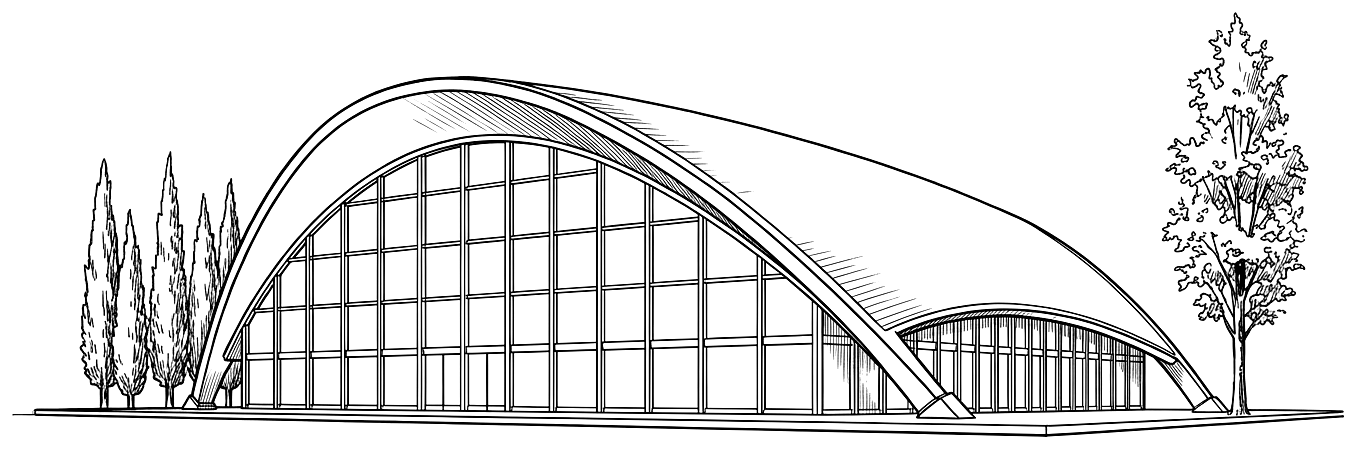
\includegraphics[width=0.78\textwidth]{fig_007_3.png}
  \caption*{图\ 7.3}
\end{figure}

\begin{figure}[htbp]
  \centering
  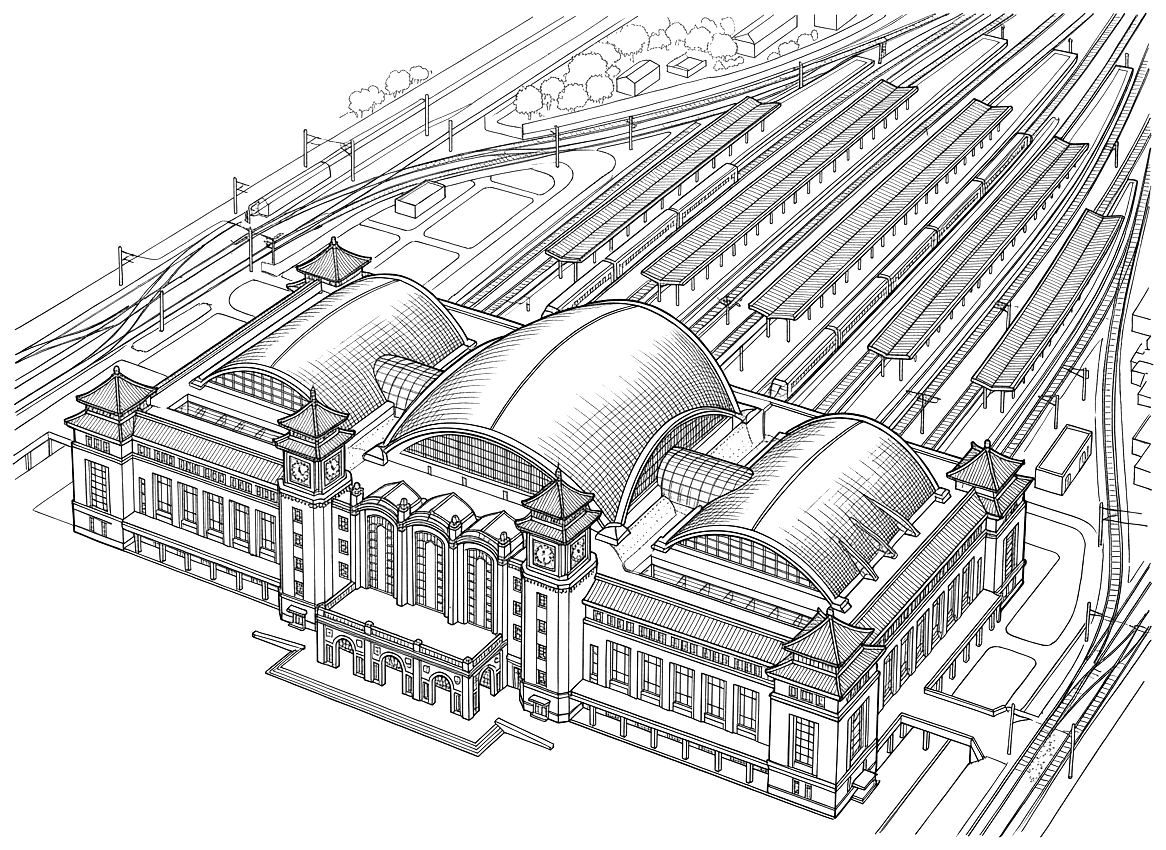
\includegraphics[width=0.78\textwidth]{fig_007_4.png}
  \caption*{图\ 7.4}
\end{figure}
